\chapter{ТЕХНОЛОГИЧЕСКАЯ ЧАСТЬ}
\label{cha:ch_3}

Технологическая часть дипломного проекта заключается в разработке технологического процесса производства детали <<Днище двигательной установки>>

\section{Общая часть}

\subsection{Назначение детали}
Деталь является передним днищем двигателя, препятствующим прорыв продуктов сгорания твердого топлива в сторону вычислительного блока управляемой ракеты. Деталь должна держать 14 атмосфер в течении 4 секунд во время работы РДТТ на режиме. Днище соединяется резьбой с обечайкой двигателя, корпус ракеты соединяется с деталью четырьмя болтами. Также в отверстие в детали вкручивается воспламенитель двигателя твердого топлива.
Предъявляются требования к герметичности соединения детали с обечайкой двигателя и с воспламенителем. Также к детали предъявляются требования по массе с целью увеличения массы полезной нагрузки управляемой ракеты.

Материал детали - сталь 33Х3СНМВФА (сплав СП-33).

\subsection{Материал детали и его свойства}
Сталь 33Х3СНМВФА относится к классу легированной конструкционной стали. Сталь широко используется для изготовления поковок. Еще из нее производят цельнокатаные кольца, служащие для производства разнообразных деталей энергетического и тяжелого машиностроения.
Химический состав стали (в \%) представлен в таблице \ref{tab:techno_steel}.
\begin{table}[h]
	\begin{center}
		\caption{}
		\begin{tabular}{|l|l|l|l|l|l|l|l|}
		\hline
C & Si & Mn & Ni & S & P & Cr & Cu \\ \hline
0,28 - 0,34 & 0,9 - 1,2 & 0,8 - 1,1 & до   0,3 & до   0,025 & до   0,025 & 0,8 - 1,1 & до   0,3 \\ \hline
		\end{tabular}
		\label{tab:techno_steel}
	\end{center}
\end{table}

Физические свойства стали 33Х3СНМВФА:

твердость материала, HB  = 65 МПА.

\begin{table}[h]
	\begin{center}
		\caption{}
		\begin{tabular}{|l|l|l|l|l|l|l|l|}
		\hline
T &  $E \cdot 10^5 $ & $\alpha \cdot 10^6 $ & l  &   $\rho$ & C & $R \cdot 10^6 $   \\ \hline
Град & МПа & 1/Град & Вт/(м$\cdot$град) & кг/м3 & Дж/(кг$\cdot$град) & Ом$\cdot$м \\ \hline
20 & 2,15 &  & 38 & 7850 &  & 210 \\ \hline
100 & 2,11 & 11,7 & 38 & 7830 & 496 & \\ \hline
		\end{tabular}
		\label{tab:techno_steel}
	\end{center}
\end{table}

T - температура, при которой получены данные свойства, °C;

E - модуль упругости первого рода, МПа;

$\alpha$ - коэффициент температурного (линейного) расширения (диапазон 20° - T), 1/°C;

l - коэффициент теплопроводности (теплоемкость материала), Вт/(м$\cdot$°C);

$\rho$ - плотность материала, кг/$\text{м}^3$;

C - удельная теплоемкость материала (диапазон 20° - T), Дж/(кг$\cdot$°C);

R - удельное электросопротивление, Ом$\cdot$м.

\subsection{Выбор вида и метода получения заготовки}
Исходя из конструкции изделия и годового объема выпуска (мелкосерийное производство), для детали <<Днище двигательной установки>> целесообразно использовать штампованную заготовку. Это позволит повысить коэффициент использования материала и снизить объем механической обработки.

Учитывая опыт создания подобных деталей, требования к прочностным свойствам детали и механические свойства материала, для получения заготовки был выбран метод горячей объемной штамповки.

\subsection{Расчет припусков на механическую обработку}
Припуск – слой материала, назначаемый для компенсации погрешностей, возникающих в процессе изготовления детали, в целях обеспечения заданного ее качества. Различают минимальные, номинальные и максимальные припуски на обработку. Они удаляются с поверхности заготовки в процессе ее обработки для получения детали.

Рассчитаем припуски на механическую обработку для получения размеров штамповки.

Качество поверхности поковки для метода горячей объемной штамповки Rz = 80 мкм, h = 150 мкм (\cite{TECHNO}, стр. 186, табл. 12).

Габаритный размер детали 125 мм.

Для определения припуска стальных заготовок, изготовляемых методами объемной горячей штамповки, используется зависимость:
$$Z = K_\text{точн} \cdot K_\text{мат} \cdot K_\text{сл} \cdot m_\text{д}^0.1544 \cdot L_H^0.27 \cdot R_\alpha^-0.0238 $$

$K_\text{точн}$ - коэффициент, учитывающий квалитет точности (для данной детали $K_\text{точн}$ = 1);

$K_\text{сл}$ – коэффициент сложности штамповки в зависимости от С1 и С2, в нашем случае $K_\text{сл}$ =1;

$K_\text{мат}$ – коэффициент, учитывающий вид материала заготовки. Наш материал по данной градации относится к М2, следовательно $K_\text{мат}$ = 1,1528;

$m_\text{д}$ – масса детали = 0,35 кг;

$L_H$ – габаритный размер элемента детали;

$R_\alpha $ = 1,6 – шероховатость размерной обработки;

\clearpage
\section{Технологический процесс изготовления детали}

\subsection{Технологический процесс}
Маршрутная карта технологического процесса производства изделия «Болт» представлена в приложении \ref{chapter:appendix_techno} (страница \pageref{chapter:appendix_techno}).

\subsection{Термическая обработка}
В процессе изготовления деталь подвергается термообработке, которая включает в себя:
\begin{enumerate}[1.]
	\item Закалка:
	\begin{itemize}
		\item Температурa: $900 \pm 20$ \textdegree C 3 минуты
		\item Среда нагрева: расплав хлористого калия;
		\item Среда охлаждения: щелочь.
	\end{itemize}
	\item Отпуск при температуре $600 \pm 20 $ \textdegree С 20 минут
	\begin{itemize}
		\item Температурa: $ 600 \pm 20 $ \textdegree С 20 минут
		\item Среда нагрева: воздух;
		\item Среда охлаждения: воздух.
	\end{itemize}
\end{enumerate}

Закалка выполняется в приспособлении, расстояние между деталями не менее 10 мм. Загрузка в сетках запрещается. Щелочную ванну раскислять желтой кровяной солью в количестве 0,1\% от веса расплава. Перед термообработкой заготовки необходимо обезжирить. После закалки необходимо промыть заготовки в горячей воде до полного удаления остатков щелочи. График температуры закалки представлен на рисунке \ref{fig:techno_termogr}.

После обработки проверить твердость HRС=35,5..40,5 на образце свидетеле по ГОСТ 22975-78. Использовать твердометр ТР 5000А

\begin{figure}[h]
	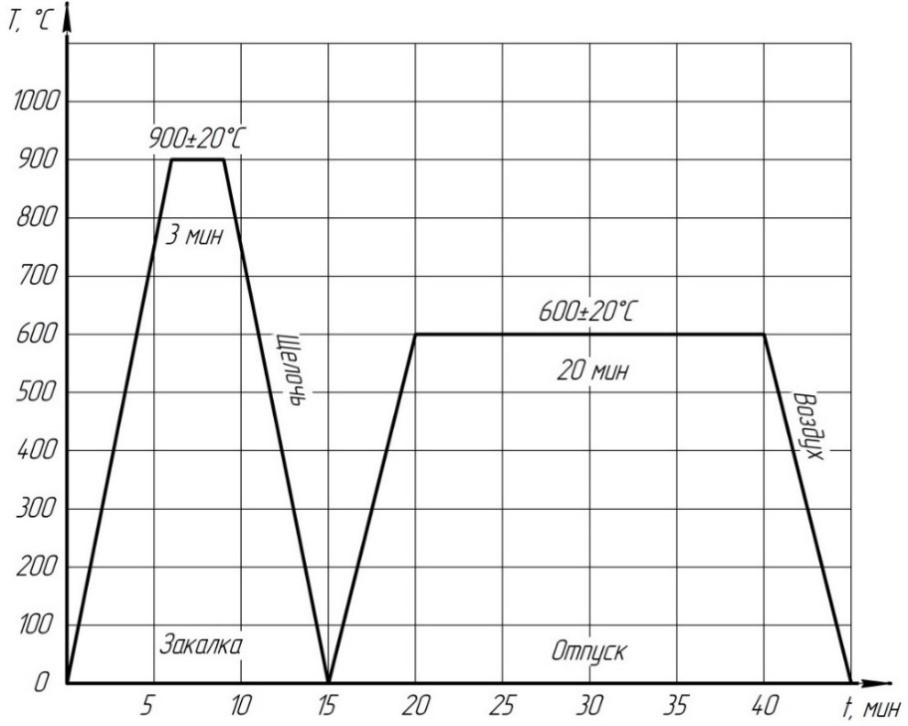
\includegraphics[width=\linewidth]{techno_termogr}
	\caption{График термической обработки}
	\label{fig:techno_termogr}
\end{figure}

\subsection{Расчет режимов механической обработки}

\paragraph{Точение}

\paragraph{Определение глубины резания $t$, мм}

Цилиндрическая поверхность диаметром $\varnothing$ 126 мм точится до $\varnothing$ 27 (операция №1, переход 7). Припуск равен t = 0.25 мм (на сторону).  Так как заданный параметр шероховатости Rz = 20 мкм (точение черновое), то точение выполняется в 1 проход, и глубина резания составляет t = 0,25 мм. 

\paragraph{Определение подачи $S$, мм/об.}

Величина подачи определяется заданным уровнем шероховатости, направлением подачи и обрабатываемым материалом. 33Х3СНМВФА.
$ s = 0.33 $ мм/об (табл.12, стр. 267 \cite{TECHNO}).

\paragraph{Скорость резания V, м/мин}

При растачивании скорость резания, рассчитывается по формуле:
$ V = \frac{C_V}{T^m t^x S_Y}$,   где

$K_V$ – поправочный коэффициент для скорости резания. $K_V = K_{MV} \cdot K_\text{ПV} \cdot K_\text{ИV}$ .

$K_\text{MV} $  – зависит от качества обрабатываемого материала.

Для 33Х3СНМВФА:	    (табл.3 стр.263 \cite{TECHNO}),

$K_\text{пv}$ – зависит от состояния поверхности ($K_\text{пv} = 0,8$ – штамповка, $K_\text{пv} = 1$ – без корки (табл.5 стр.263 \cite{TECHNO})):	$K_\text{пv} = 1,0$;

$K_\text{ИV}$ – зависит от материала инструмента (табл.6 стр.263 \cite{TECHNO}).

$K_\text{ИV} = 0,5$ – инструмент из твердого сплава ВК6, обрабатываемый материал сталь 33Х3СНМВФА.

$$K_V = 1.0 \cdot 1,0 \cdot 0,5 = 0,5$$

T, мин – стойкость резца.  Для токарной обработки принять  T = 50 мин.

Коэффициенты и показатели степени в соответствии с табл.17 \cite{TECHNO}:
– для  $s \le 0,4$   мм/об:

CV = 292, y = 0,20, x = 0,15, m = 0,20 (твердый сплав).

 $ V = \frac{292}{50^0,2 0,5^0,15 0,3_0,2} \cdot 0,5 = 94,2 $ м/мин.

\paragraph{Частота вращения шпинделя n об/мин} По установленной скорости резания определяем частоту вращения шпинделя
$ n = \frac{1000 \cdot V } { \pi \cdot D} $, где

D – диаметр обрабатываемой поверхности. Частота вращения должна быть не изменой в рамках одного перехода, поэтому рассчитывается для максимальных значений D поверхностей обрабатываемых в данном переходе.
Полученные значения округляются в соответствии с паспортными данными станка (обычно в сторону занижения). 
$ n = \frac{1000 \cdot 94,2} { 3,14 \cdot 30} =1000 $ об/мин.

Пересчитываем скорость резания при чистовом точении с учётом изменившейся частоты вращения:

$ V = \frac{n \pi D}{1000} = \frac{1000 \cdot pi \cdot 27} {1000} = 84,2$ м/мин.

\paragraph{Технологическое (основное) время  $Т_\text{ОСН}$, мин}

$Т_\text{ОСН} = \frac{L \cdot 2 } {S \cdot n}$ , где
L – расчетная длина рабочего хода режущего инструмента, т.е. путь, проходимый режущим инструментом в направлении подачи, мм.

$Т_\text{ОСН1} = \frac{77 \cdot 2 } {0.3 \cdot 1000}$ мин.

Примем $Т_\text{всп}$ = 0,5 мин, $Т_\text{пз}$= 5  мин для всех режимов.

\clearpage
\paragraph{Сила резания $P_Z$, Н. Эффективная мощность $N$, кВт}

$$P_Z = 10 C_p \cdot t^X \cdot S_Y \cdot V^n \cdot K_p$$

Коэффициенты и показатели степеней:

CP = 300, y = 0,75, x = 1, n = 0 (материал режущей части резца – ВК6) табл. 22 стр.273 \cite{TECHNO}.

	$K_{MP} = 0,75$ ; $K_\text{ФР} = 0,89$ ; $K_{\gamma P} = 1,1$ ; $K_{\lambda P} = 1,0 $  ; $K_{rp} = 1.0 $

	$$K_P = 0,75 \cdot 1,1 \cdot 0,89 \cdot 1 \cdot 1 = 0,74$$

Черновое точение $P_Z1 = 2396$  Н,

$ N = \frac{2400 \cdot 60} { 60000} = 2,4 $ кВт.

Установленные значения $P_z$ и $N$ не превышают усилия резания, допускаемого механизмом подачи станка, и эффективной мощности на шпинделе станка. Следовательно, выбранный режим осуществим.
Для обработки используется проходной упорный резец изготовленный из твердого сплава ВК6, обладающей повышенной прочностью и пригодного для изготовления режущего инструмента всех видов, в том числе для обработки обычных конструкционных материалов в условиях динамических нагрузок. В химический состав сплава входят 94\% корбида вольфрама, 6\% кобальта.

\paragraph{Сверление}

Определение глубины резания $t,$ мм.

Сверлится отверстие $\varnothing$  4 мм. При сверлении глубина резания равна $t = 0,5 \cdot D = 0,5 \cdot 4 = 2$ мм.

\paragraph{Определение подачи S, мм/об}

Величина подачи без ограничивающих факторов определяется твёрдостью материала детали и диаметром сверла. Для сверла $\varnothing$  4 мм и материала 33Х3СНМВФА выбираем подачу  s = 0,21 об/мин (табл. 25, стр. 277 \cite{TECHNO}).

\paragraph{Скорость резания V, м/мин}

Скорость резания при сверлении определяется формулой:  $ V = \frac { C_V \cdot D^q} { T_m \cdot S^Y} \cdot K_V$.

KV – поправочный коэффициент для скорости резания.

$K_V$ – поправочный коэффициент для скорости резания. $K_V = K_{MV} \cdot K_\text{tV} \cdot K_\text{ИV}$ .


$K_{MV}$  – зависит от качества обрабатываемого материала.

Для 33Х3СНМВФА: $K_{MV} = 1,1$    (табл.3 стр.263 \cite{TECHNO}),

$K_\text{ИV}$ – зависит от материала инструмента (табл.6 стр.263 \cite{TECHNO}).

$K_\text{ИV} = 1,0$ – инструмент из Р6М5, обрабатываемый материал 33Х3СНМВФА,

$K_\text{tV}$  – коэффициент, учитывающий глубину сверления (табл.31 стр.280\cite{TECHNO}).

$K_\text{tV} $=0,5 – отверстие имеет глубину 5.

$K_\text{V} = 1,0 \cdot 1,0 \cdot 0,5 = 0,55$;

T, мин – стойкость резца.  Для обработки сверлением принять  T = 25 мин (табл.30 стр.280 \cite{TECHNO}).

Коэффициенты и показатели степени в соответствии с табл.28 \cite{TECHNO}:
– для $s \le 0,2 $    мм/об:

$C_V$ = 7,0, y = 0,7, q = 0,4, m = 0,2 (быстрорежущая сталь Р6М5).

$$ V = \dfrac{ C_V \cdot D^q} {T^m \cdot S^y} \cdot K_V = \dfrac{7,0 \cdot 0,5^{0,4}}{25^{0,25} \cdot 0,21^{0,7}} \cdot 0,5 = 11,615 $$
 
\paragraph{Частота вращения шпинделя n об/мин}
По установленной скорости резания определяем частоту вращения шпинделя
 $n = \frac{1000 \cdot V}{\pi \cdot D}, n = 500 $ об/мин.

Пересчитываем скорость резания и получаем $V = 9,5$ м/мин .

\paragraph{Технологическое (основное) время  ТОСН, мин}

$ T_\text{ОСН} = \frac{L}{S\cdot n, T_\text{ОСН} = 0,9 } $ мин.

Примем $Т_\text{всп}$ = 0,5 мин,$ Т_\text{пз} $= 5  мин для всех режимов.

\paragraph{Крутящий момент Мкр, Н*м и осевая сила  P, Н.}

Данные характеристики сверления находят по формулам:
$$M_KP = 10 \cdot C_M \cdot D^q \cdot s^Y \cdot K_p ; P_0 = 10 \cdot C_p \cdot D^q \cdot s^Y \cdot K_p$$

Значения коэффициентов $C_M$  и $C_p$  и показателей степени приведены в табл. 32 \cite{TECHNO}. Коэффициенты и показатели степени в формулах крутящего момента: $C_M = 0,0345$ , q=2,0, y=0,8.

Коэффициенты и показатели степени в формулах осевой силы:
$C_p = 68$ , q=1,0, y=0,7.

Коэффициент, учитывающий фактические условия обработки, в данном случае зависит только от материала обрабатываемой заготовки и определяется выражением: $K_P = K_MP$ .

Для конструкционных сталей коэффициент $K_MP = 0,75$  (табл.10 стр.265 \cite{TECHNO}), след. $K_P$ = 0,75 .

$M_{KP} = 10 \cdot 0,0345 \cdot 6^2 \cdot 0,2^0,8 \cdot 0,75 = 2,57$ Н * м;

$P_O = 992 $ Н.

\paragraph{Мощность резания  Nр, кВт.}
Мощность резания определяют по формуле:

$$ N_p = \frac{M_kp \cdot n} { 9750} = \frac{2,57 \cdot 530} {9750} = 0,14 \text{ кВт}.$$

Допустимый крутящий момент на шпинделе станка и эффективная мощность превышает установленные расчетные значения. Следовательно, выбранный режим осуществим.
